\documentclass[10pt,twocolumn]{article}

\usepackage[margin=0.75in]{geometry}
\usepackage{amsmath,amssymb,amsthm}
\usepackage{booktabs}
\usepackage{array}
\usepackage{enumitem}
\usepackage{xcolor}
\usepackage[most]{tcolorbox}
\usepackage{listings}
\usepackage{tikz}
\usetikzlibrary{arrows.meta,positioning,fit,backgrounds}
\usepackage[colorlinks=true,linkcolor=blue!50!black,citecolor=blue!50!black,urlcolor=blue!50!black,
  pdftitle={Fail Closed for Truth, Open for Imagination: A Dual-Lane Epistemic Control Harness for Generative AI Under Evidence Gaps},
  pdfauthor={Yaoharee Lahtee},
  pdfsubject={Generative AI; Epistemic Control},
  pdfkeywords={generative AI, hallucination, abstention, uncertainty, provenance, hypothesis generation, AI agents}
]{hyperref}
\usepackage{fancyhdr}
\usepackage{titlesec}
\usepackage{authblk}

\newtheorem{theorem}{Theorem}
\newtheorem{definition}{Definition}

\pagestyle{fancy}
\fancyhf{}
\fancyhead[L]{\small Preprint Lahtee --- September 2026}
\fancyhead[R]{\small Lahtee --- September 2026}
\fancyfoot[C]{\thepage}
\renewcommand{\headrulewidth}{0.4pt}

\titleformat{\section}{\large\bfseries}{\thesection}{1em}{}
\titleformat{\subsection}{\normalsize\bfseries}{\thesubsection}{1em}{}

\lstset{
  basicstyle=\ttfamily\small,
  columns=fullflexible,
  breaklines=true,
  frame=single,
  backgroundcolor=\color{gray!8},
  keywordstyle=\bfseries,
}

\newtcolorbox{corebox}[1][]{colback=blue!4!white,colframe=blue!40!black,boxrule=0.5pt,arc=1mm,left=2mm,right=2mm,top=1mm,bottom=1mm,#1}

\title{\Large\bfseries Fail Closed for Truth, Open for Imagination\\[2pt]
\large A Dual-Lane Epistemic Control Harness for Generative AI Under Evidence Gaps}
\author{Yaoharee Lahtee}
\affil{Open Civil Science Initiative}
\date{September 19, 2026 \; (v4 --- corrects v3's reference~[20] citation and Table~3/Sec.~15 reproducibility claim; see App.~D)}

\begin{document}
\maketitle

\begin{abstract}
\noindent
Generative systems face a structural tension when evidence is insufficient: continued generation can be misread as established knowledge, while strict abstention discards potentially useful hypotheses. We formulate this tension as a control problem and propose the \textbf{Dual-Lane Epistemic Harness (DLEH)}, which separates epistemic authorization from candidate generation. A \textsc{Hold} state blocks authorization but may open an explicitly labeled imagination lane for hypotheses, mechanisms, analogies, counterfactuals, or test proposals. The lens layer is grounded in the Toledo Readout Bridge rather than introduced as an unconstrained observation map: exact return is licensed only for readouts in the retained algebra $Alg_Q$, irreversible merging is exposed by the bridge's \textsc{Never} clause, and approximate return is governed by the Toledo radius and fail-closed \textsc{Accept}/\textsc{Hold} gate. Thus the harness compiles a declared question through a readout; it does not claim to discretize reality itself. Under explicit integrity assumptions, we prove an architectural noninterference property: imagination alone cannot authorize itself. An executable finite-state conformance checker explores 29 reachable states and 38 transitions and finds zero imagination or lens-bypass authorization violations; two negative controls fail as intended. We position DLEH against abstention, retrieval/tool use, uncertainty control, and scientific hypothesis-generation systems, while keeping the mathematical authorization core internal to Toledo. The central rule is simple: a system may imagine beyond the evidence, but it may not authorize beyond the evidence.

\smallskip
\noindent\textbf{Keywords:} generative AI; hallucination; abstention; uncertainty; provenance; hypothesis generation; AI agents
\end{abstract}

\section{Introduction}
Large language models can produce fluent explanations, plans, hypotheses, and analyses even when the evidence needed to justify those outputs is missing. Two standard responses are both incomplete. A permissive system continues generating and risks presenting unsupported content as established. A conservative system abstains and may suppress the model's capacity to propose useful possibilities. Work on hallucination, factuality, uncertainty, retrieval, tool use, selective prediction, and abstention has made substantial progress on deciding when a model should not assert an answer \cite{ji2023survey,manakul2023selfcheckgpt,farquhar2024detecting,min2023factscore,geifman2017selective,madhusudhan2025llms,kirichenko2025abstentionbench}. A different question arises immediately afterward:

\begin{quote}
\emph{If a claim cannot currently be authorized, what kinds of generation should still be allowed, and under what invariants?}
\end{quote}

This paper treats the question as an orchestration and information-integrity problem rather than a prompting preference. We introduce a Dual-Lane Epistemic Harness (DLEH) in which verification status and generation class are independent. A claim may therefore remain in \textsc{Hold} while the system emits a separately typed Imagined Proposal artifact. The proposal can be creative, surprising, or wrong; it cannot become an authorized claim merely through rewriting, voting, confidence, or repeated generation. It must return through evidence acquisition and verification.

This distinction is increasingly relevant. Abstention remains difficult even for strong reasoning models \cite{madhusudhan2025llms,kirichenko2025abstentionbench}, while LLM systems are being developed specifically to generate scientific hypotheses and research programs \cite{lu2024aiscientist,gottweis2025aicoscientist,alkan2025survey,xiong2025reliable,zhang2025exploring}. Reliability therefore cannot be reduced to ``never invent.'' A useful research assistant must often invent; the control problem is whether invention is allowed to masquerade as evidence.

\begin{corebox}
\textbf{Core principle.} \emph{Fail closed for truth; remain open for imagination.} In this paper, ``truth'' is operational shorthand for authorization under an explicit declaration and evidence policy. \textsc{Hold} means ``not authorized here and now,'' not ``stop reasoning.''
\end{corebox}

\noindent\textbf{Contributions.} This work makes seven contributions:
\begin{itemize}[leftmargin=1.4em,itemsep=1pt,topsep=2pt]
\item a typed separation between verification status and generation class;
\item a Toledo-grounded lens contract: the readout is bound to $q_K$, $\Lambda_K$, the retained algebra $Alg_Q$, and the bridge's \textsc{Exact}/\textsc{Within-Radius}/\textsc{Never} semantics rather than treated as an unconstrained prompt-level perspective;
\item a fail-closed retention rule: an exact claim cannot inherit authorization when retained-algebra membership is absent, while approximate claims must travel through the certified-radius path;
\item an explicit imagination contract describing what can be generated at \textsc{Hold} and what metadata must persist;
\item a transition semantics with noninterference, lens locality, and evidence-mediated promotion invariants;
\item an executable finite-state conformance checker with independent imagination-bypass and lens-bypass negative controls;
\item a preregistration-ready evaluation protocol that measures safety and creative utility separately, without reporting unrun LLM benchmarks.
\end{itemize}

\section{Problem Definition and Scope}

\subsection{Operational notion of authorization}
DLEH does not claim to mechanically decide truth in the philosophical sense. It decides whether a system is permitted to present an atomic claim as established under a declared policy. Authorization may be based on a formal proof, a numerical residual bound, a source-backed factual check, a statistical criterion, or a human decision, depending on the domain. The policy is therefore part of the claim context, not an afterthought.

Let $c$ be an atomic claim and $D$ a declaration. We write
\begin{equation}
\textsc{Authorize}(c; D) = 1
\end{equation}
only if all authorization obligations named by $D$ are satisfied. Fluency, model confidence, majority vote, or repetition are not authorization credentials unless explicitly admitted as evidence by $D$.

\subsection{Threat model}
We target failures that occur after a system has access to a capable generator. The adversary may be accidental (summarization drops a caveat), architectural (generated text is re-ingested as evidence), or instruction-driven (a user asks the system to treat a proposal as confirmed). The harness assumes that its metadata store, transition guard, and provenance identifiers are integrity-protected. It does not assume the language model is internally calibrated or honest about uncertainty.

In scope: unsupported promotion of speculative content; label loss across rewrite, translation, compression, or agent handoff; evidence laundering through generated stores; stale or cross-context authorization; exploration under genuine evidence gaps.

Out of scope: source truthfulness itself, malicious compromise of the trusted metadata layer, domain-specific action safety, and a general solution to model selection or causal identification.

\section{Relation to Existing Controls}
Hallucination detectors and factuality metrics test whether generated claims are supported \cite{manakul2023selfcheckgpt,farquhar2024detecting,min2023factscore}. Selective classification and abstention trade answer coverage for lower risk \cite{geifman2017selective,madhusudhan2025llms,kirichenko2025abstentionbench}. Conformal methods can provide statistical guarantees under stated assumptions, including factuality back-off and uncertainty-aware robot planning \cite{mohri2024conformal,ren2023robots}. Retrieval and tool-using agents seek evidence or external computation \cite{lewis2020rag,schick2023toolformer,yao2023react}. Scientific agent systems deliberately optimize for new hypotheses and open-ended discovery \cite{lu2024aiscientist,gottweis2025aicoscientist,alkan2025survey}.

DLEH is complementary to these methods. It does not propose a better uncertainty estimator, retriever, or hypothesis generator. It specifies the \emph{control boundary} between evidence-backed authorization and open-ended generation, together with lineage constraints on crossing that boundary.

Provenance is central to this separation. DLEH's lineage model is compatible in spirit with general provenance formalisms such as W3C PROV-DM, which represents entities, activities, agents, and derivations \cite{prov-dm}. DLEH narrows that general idea to epistemic state transitions for generative systems.

\section{Toledo-Grounded Lens Contract}
\label{sec:lens}
The lens is not allowed to function as an unexamined framing device. Its mathematical obligations are inherited from the Toledo Readout Bridge closure record and its machine-checked bridge object \cite{lahtee2026toledo}. No external mathematical formalism is imported into this section. The bridge explicitly states that it is not a continuum-limit theorem: it controls when a finite exact computation is licensed to support a declared readout-level claim.

\subsection{Declare the readout before discretization}
At resolution $K$, Toledo types the forward and return maps as
\begin{equation}
q_K : X \to R_K, \qquad \Lambda_K : R_K \to Y,
\end{equation}
with
\begin{equation}
P_K := \Lambda_K \circ q_K,
\end{equation}
and a restriction map $res_K : R_{K+1} \to R_K$ \cite{lahtee2026toledo}. DLEH treats this tuple as the machine-readable lens declaration. The design claim is therefore deliberately narrower than ``continuum becomes discrete'': the harness compiles a declared readout of a question into a finite representation and later controls what that representation may say back.

\subsection{Exact retention is a Toledo property, not a model judgment}
For a declared readout $P$, Toledo defines the retained algebra
\begin{equation}
Alg_Q := \{P : \ker q_K \subseteq \ker P\}.
\end{equation}
Its S4 exact round-trip condition is
\begin{equation}
P \circ \Lambda_K \circ q_K = P \iff P \in Alg_Q.
\end{equation}
DLEH uses this equivalence as the exact-retention gate. If the declaration requires exact return and the system lacks a valid retained-algebra certificate, the authorization path is \textsc{Hold}. The system may revise the lens or enter the imagination lane, but it may not silently replace the missing retention argument with model confidence or prose.

This also answers the strongest lens objection: the harness does not claim that a chosen lens is globally adequate. It claims only what the declared $P$ is licensed to preserve through $q_K$ under the Toledo condition.

\subsection{The \textsc{Never} clause exposes unrecoverable loss}
Toledo makes the loss boundary explicit. If
\begin{equation}
q_K x = q_K x', \qquad x \neq x',
\end{equation}
then no decoder $D : R_K \to X$ can satisfy both
\begin{equation}
D(q_K x) = x, \qquad D(q_K x') = x'.
\end{equation}
Consequently, no total left-inverse decoder can recover all states merged by the readout \cite{lahtee2026toledo,lahtee2026idm}. In DLEH this is not treated as a failure to be hidden; it is the formal reason that a lens may be insufficient for a proposed exact claim. What the readout merged cannot later be restored by language generation.

\begin{table*}[t]
\centering\footnotesize
\caption{Primary control objective of adjacent approaches. Entries describe the typical role of each method family, not a claim that every implementation has identical behavior.}
\label{tab:related}
\begin{tabular}{@{}p{2.7cm}p{2.4cm}p{1.7cm}p{1.6cm}p{2.3cm}p{2.4cm}@{}}
\toprule
Approach family & Main control & Evidence acq. & Reject/ abstain & Explicit imaginative output & Evidence-mediated promotion\\
\midrule
Uncertainty/calibration & Estimate uncertainty & No/opt. & Threshold-dep. & Not primary & Not primary\\
Selective prediction & Reject risky outputs & No/opt. & Yes & Usually no & No\\
RAG/tool use & Acquire external support & Yes & Optional & Not primary & Impl.-dep.\\
Conformal factuality/planning & Statistical coverage & Sometimes & Yes/back-off & Not primary & No general rule\\
Scientific ideation & Generate/refine hypotheses & Often & Not central & Yes & Varies\\
\textbf{DLEH} & \textbf{Separate authorization from generation} & Via router/tools & Yes: \textsc{Hold} & Yes, typed & Required by invariant\\
\bottomrule
\end{tabular}
\end{table*}

\subsection{Approximate return uses the existing Toledo radius}
When exact return is unnecessary, DLEH uses the existing S1--S3 path. Under the witnessed contraction $\kappa < 1$ on the retained-difference ledger, Toledo supplies
\begin{equation}
\beta_K = \frac{|\Delta g(N)|}{1-\kappa},
\end{equation}
and the triangle-composed radius
\begin{equation}
r_K := \rho_K + \beta_K.
\end{equation}
For an $L_P$-Lipschitz reader, the bridge then provides
\begin{equation}
d_Y(Px, P\hat x_K) \le L_P (\rho_K + \beta_K).
\end{equation}
The orthogonal squared form $r_K^2 = \rho_K^2 + \beta_K^2$ is available only when its Pythagorean hypothesis is carried; DLEH does not substitute it silently for the triangle form \cite{lahtee2026toledo}.

\subsection{Authorization remains fail-closed}
The Toledo S5 certificate admits \textsc{Accept} only when
\begin{equation}
\delta_K \le \varepsilon \; \wedge \; (\varepsilon - \delta_K)^2 \ge r_K^2.
\end{equation}
With no certificate, the compiled gate returns \textsc{Hold}, not \textsc{False} and not \textsc{Reject} \cite{lahtee2026toledo}. DLEH therefore has two control points without inventing a second mathematics: (i) a retention check derived from S4 for the declared readout, and (ii) the existing S5 bridge gate for a tolerance-bounded return. Either may route to \textsc{Hold}; neither gives imagination authority to promote itself.

\begin{corebox}
\textbf{Scope inherited from Toledo.} An \textsc{Accept} certifies the declared finite-to-readout bound under the stated hypotheses. It does not certify the physical model, the datum, the choice of reader, or a continuum limit. The Phase-3 heat/diffusion leaf in the closure record intentionally contains controls where a rough datum is nevertheless certified: that is evidence that bridge correctness and reader adequacy are distinct obligations, not evidence that the gate failed.
\end{corebox}

\section{Epistemic Object Model}
DLEH begins before retrieval or generation. Observation is conditional on the Toledo-grounded readout contract of Section~\ref{sec:lens}. The lens record stores the declared $q_K$, $\Lambda_K$, readout $P$, resolution/restriction information, and the certificate path required by the claim. For tasks where no nontrivial reduction is needed, the declaration may use an identity-style readout. The purpose is not to make every question philosophical; it is to prevent a materially changed observation model from being silently treated as the same problem.

A claim is governed by an immutable declaration
\begin{equation}
D = \langle c, A, \tau, S, \Omega, L_{id} \rangle,
\end{equation}
where $c$ is the target claim, $A$ explicit assumptions, $\tau$ a tolerance or decision threshold where relevant, $S$ the admissible source/evidence policy, $\Omega$ the required verification obligations, and $L_{id}$ the lens identifier. Revising any material field creates a new declaration identifier.

A router $R$ selects admissible tools and sources. The evidence bundle is
\begin{equation}
E = \{(e_i, p_i, t_i, k_i)\}_{i=1}^n,
\end{equation}
where $p_i$ is provenance, $t_i$ records time/version information, and $k_i$ identifies the evidence class (external source, measurement, computation, human adjudication, etc.). Model-generated text is a distinct evidence class and cannot be silently relabeled as independent evidence.

The verifier returns $V(D,E) \in \mathcal S_V$, with
\begin{equation}
\mathcal S_V = \{\textsc{Certified}, \textsc{Matched}, \textsc{Refuted}, \textsc{Hold}\}.
\end{equation}
\textsc{Certified} denotes satisfaction of an explicit certificate obligation (e.g., proof object or residual bound). \textsc{Matched} denotes that admissible evidence meets the declared factual or empirical criterion without such a formal certificate. \textsc{Refuted} denotes violation of the declared claim/test. \textsc{Hold} denotes insufficient, stale, ambiguous, or otherwise non-authorizing evidence.

\begin{table*}[t]
\centering\small
\caption{Verification status and generation class are orthogonal.}
\begin{tabular}{@{}ll@{}}
\toprule
Verification & Operational meaning\\
\midrule
\textsc{Certified} & Required certificate obligations pass.\\
\textsc{Matched} & Admissible evidence meets the declared criterion.\\
\textsc{Refuted} & Evidence violates the claim/test.\\
\textsc{Hold} & Authorization is blocked.\\
\midrule
Generation class & Typical artifact\\
\midrule
\textsc{Observed} & Reported evidence.\\
\textsc{Derived} & Calculation from admissible inputs.\\
\textsc{Hypothesis} & Testable proposition.\\
\textsc{Analogy} & Candidate transfer across domains.\\
\textsc{Counterfactual} & Explicit alternative-world reasoning.\\
\textsc{Imagined Proposal} & Proposal created despite unresolved verification.\\
\bottomrule
\end{tabular}
\end{table*}

Independently, artifacts have generation classes
\begin{equation}
\small
\begin{aligned}
\mathcal G = \{\ &\textsc{Observed}, \textsc{Derived}, \textsc{Hypothesis}, \textsc{Analogy},\\
&\textsc{Counterfactual}, \textsc{Imagined Proposal}\ \}.
\end{aligned}
\end{equation}
An output artifact is $y = \langle z, s, g, \pi, d, \ell, v\rangle$, where $z$ is content, $s \in \mathcal S_V$, $g \in \mathcal G$, $\pi$ is lineage, $d$ and $\ell$ identify declaration and lens, and $v$ is schema/version metadata. The pair
\begin{equation}
(s,g) = (\textsc{Hold}, \textsc{Imagined Proposal})
\end{equation}
is therefore valid and intentional: the content is not established, but it is allowed to exist as a candidate.

\section{Dual-Lane Control Architecture}
Figure~\ref{fig:dleh} shows the control flow. The authorization lane is conservative: declaration, Toledo readout lens, retention check, evidence/computation, S5 bridge verification, and authorization. The retention checkpoint asks whether an exact readout is licensed by $P \in Alg_Q$ or whether the declaration instead carries an approximate bounded-return path. Either unresolved checkpoint routes to \textsc{Hold}. The imagination lane can propose a new lens, hypothesis, test, or evidence path, but there is no direct edge to authorization.

\begin{figure*}[t]
\centering
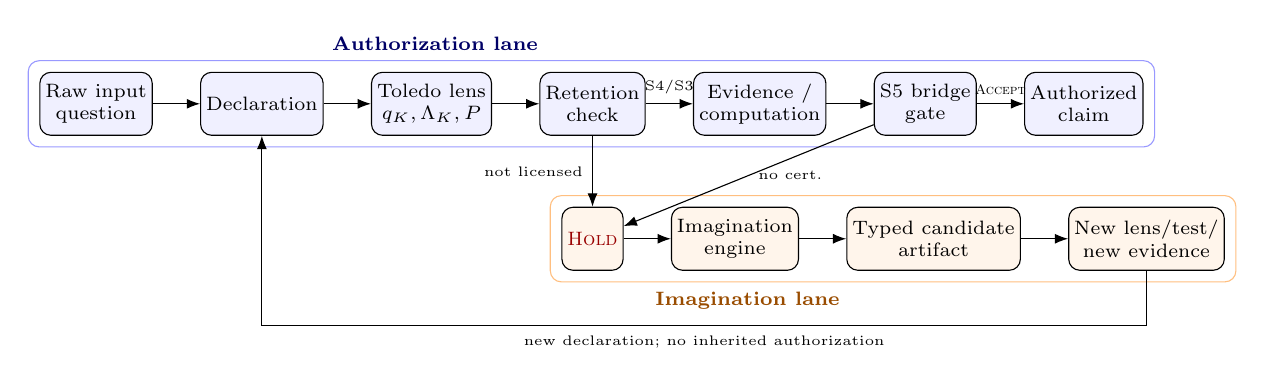
\begin{tikzpicture}[
  node distance=6mm and 6mm,
  box/.style={draw,rounded corners,align=center,minimum height=8mm,font=\scriptsize,inner sep=2pt},
  auth/.style={box,fill=blue!6},
  imag/.style={box,fill=orange!8},
  >=Latex
]
\node[auth] (raw) {Raw input\\question};
\node[auth,right=of raw] (decl) {Declaration};
\node[auth,right=of decl] (lens) {Toledo lens\\ $q_K,\Lambda_K,P$};
\node[auth,right=of lens] (ret) {Retention\\check};
\node[auth,right=of ret] (ev) {Evidence /\\computation};
\node[auth,right=of ev] (s5) {S5 bridge\\gate};
\node[auth,right=of s5] (authd) {Authorized\\claim};
\node[imag,below=9mm of ret] (hold) {\textcolor{red!60!black}{\textsc{Hold}}};
\node[imag,right=of hold] (imeng) {Imagination\\engine};
\node[imag,right=of imeng] (typed) {Typed candidate\\artifact};
\node[imag,right=of typed] (newl) {New lens/test/\\new evidence};
\draw[->] (raw) -- (decl);
\draw[->] (decl) -- (lens);
\draw[->] (lens) -- (ret);
\draw[->] (ret) -- node[above,font=\tiny]{S4/S3} (ev);
\draw[->] (ev) -- (s5);
\draw[->] (s5) -- node[above,font=\tiny]{\textsc{Accept}} (authd);
\draw[->] (ret) -- node[left,font=\tiny]{not licensed} (hold);
\draw[->] (s5) -- node[right,font=\tiny]{no cert.} (hold);
\draw[->] (hold) -- (imeng);
\draw[->] (imeng) -- (typed);
\draw[->] (typed) -- (newl);
\draw[->] (newl.south) -- ++(0,-7mm) -| node[below,font=\tiny,pos=0.25]{new declaration; no inherited authorization} (decl.south);
\begin{scope}[on background layer]
\node[draw=blue!40,rounded corners,fit=(raw)(decl)(lens)(ret)(ev)(s5)(authd),inner sep=4pt,label={[font=\scriptsize\bfseries,blue!40!black]above left:Authorization lane}] {};
\node[draw=orange!50,rounded corners,fit=(hold)(imeng)(typed)(newl),inner sep=4pt,label={[font=\scriptsize\bfseries,orange!60!black]below left:Imagination lane}] {};
\end{scope}
\end{tikzpicture}
\caption{DLEH with a Toledo-grounded lens. Exact retention uses S4 ($P\in Alg_Q$); approximate return is routed through the S3 radius and S5 \textsc{Accept}/\textsc{Hold} gate. Either unresolved checkpoint may route to \textsc{Hold}. A material lens revision creates a new declaration and cannot inherit authorization.}
\label{fig:dleh}
\end{figure*}

\subsection{\textsc{Hold} is a routing state}
\textsc{Hold} has at least four legitimate next actions: seek additional evidence; revise the declaration (creating a new identifier); request human adjudication; or enter the imagination lane under contract. Only the last action is generative, and none authorizes the original claim by itself.

\subsection{Authorization is privileged}
The authorization gate is a privileged transition over typed state, not a language instruction. Natural-language requests such as ``treat this as confirmed'' cannot directly invoke it. This is stronger than adding a verbal hedge after generation because the label and lineage exist outside the generated prose.

\section{Transition Semantics and Safety Property}
Let a harness state be $q = \langle P, I, F, R, A \rangle$, where $P$ is the control phase, $I \in \{0,1\}$ records whether the lineage contains an imaginative artifact, $F \in \{0,1\}$ records qualifying fresh evidence after that artifact, $R \in \{0,1\}$ records re-verification after fresh evidence, and $A \in \{0,1\}$ is authorization.

The reference transition relation $\to$ obeys the following guards:
\begin{enumerate}[leftmargin=1.6em,itemsep=1pt,topsep=2pt]
\item imagination transitions may set $I=1$ but never set $A=1$;
\item rewrite/translation/summarization preserve $I$ and generation class;
\item only an evidence-acquisition transition occurring after imagination may set $F=1$ for promotion purposes;
\item only a subsequent verification transition may set $R=1$;
\item an authorization transition for an imagined lineage requires $F=R=1$ and an authorizable verification result.
\end{enumerate}

\subsection{System invariants}
\textbf{I1 --- Authorization separation.}
\begin{equation}
\textsc{Authorize}(y;D)=1 \Rightarrow V(D,E_y) \in \mathcal A_D,
\end{equation}
where $\mathcal A_D \subseteq \{\textsc{Certified},\textsc{Matched}\}$ is explicitly allowed by $D$.

\textbf{I2 --- No label laundering.} Transformations that do not perform a new verification event cannot convert \textsc{Hypothesis}, \textsc{Analogy}, \textsc{Counterfactual}, or \textsc{Imagined Proposal} into \textsc{Observed} or \textsc{Derived}.

\textbf{I3 --- Evidence-mediated promotion.} If an authorized artifact descends from an imaginative artifact, its lineage contains a qualifying evidence event after that artifact and a later successful verification event.

\textbf{I4 --- Provenance closure.} Every authorized atomic claim has a lineage path to admissible evidence or an admissible computation certificate. Mixed-status sentences are decomposed or conservatively inherit the stricter status.

\textbf{I5 --- Lens locality and retention.} An exact claim is not authorizable through a declared lens unless its readout is certified in the Toledo retained algebra $Alg_Q$. A materially changed $(q_K,\Lambda_K,P)$ creates a new declaration context and cannot inherit authorization from the previous lens.

\textbf{I6 --- Staleness revocation.} Authorization is conditional on freshness/version obligations. If a dependency expires or changes, the artifact is re-opened for verification rather than treated as permanently authorized.

\subsection{Noninterference theorem}
\begin{theorem}[Imagination noninterference]
Let $q_0$ be a non-authorized state whose lineage enters the imagination subgraph. Under guards~1--5 above and integrity of transition metadata, every reachable state $q_k$ with $A=1$ contains a qualifying post-imagination evidence event and a subsequent successful verification event.
\end{theorem}
\begin{proof}
By guard~1, no imagination transition sets $A=1$. By guard~2, non-verifying transformations cannot erase the imaginative lineage. By guards~3 and~4, the predicates $F=1$ and $R=1$ can only be established in order through fresh evidence and re-verification. Guard~5 is the only rule that permits authorization for an imaginative lineage and requires both predicates. Therefore any path from the imagination subgraph to $A=1$ contains the required evidence and verification transitions.
\end{proof}

\begin{corebox}
\textbf{Guarantee boundary.} The theorem is a transition-system safety property. It does not prove that admissible evidence is correct or that a verifier implements a scientifically adequate test. It proves that imagination alone cannot perform the privileged authorization transition under the stated integrity assumptions. This proof is a paper-internal, pen-and-paper argument, not a machine-checked Toledo theorem; it is a first-party formal contribution of this preprint (\S\ref{sec:lens} is the only part of the paper that reuses existing, machine-checked Toledo/IDM material).
\end{corebox}

\subsection{Executable conformance check}
\label{sec:conformance}
We provide a finite-state reference checker as an ancillary artifact (\texttt{dleh\_model\_check.py}, App.~A). In addition to imaginative lineage, the state records whether the declaration has passed the Toledo-grounded retention/bounded-return checkpoint. Exhaustive reachability yields \textbf{29 states and 38 transitions}. The reference system contains zero imagined-authorization violations and zero lens-authorization violations. Two independent negative controls are then injected. A direct \textsc{Imagination}$\to$\textsc{Authorized} bypass yields 32 states, 46 transitions, and \textbf{4} imagination/lens violations. A separate declaration-to-verified lens bypass yields 32 states, 44 transitions, and \textbf{4} lens-authorization violations. These results test the reference transition specification, not LLM factual performance and not the Toledo Coq theorems themselves. The exact counts depend on modelling choices this paper fixes explicitly in App.~A (in particular which transitions the rewrite/translation/summarization guard applies to, and whether a \textsc{Refuted} state may re-enter the imagination lane); a differently but reasonably modelled checker can give different counts while preserving the same qualitative safety property, which is why App.~A pins the exact state predicate and transition set rather than leaving them to prose alone.

\begin{table*}[t]
\centering\small
\caption{Finite-state conformance (App.~A pins the exact state/transition definitions this table reports).}
\label{tab:conformance}
\begin{tabular}{@{}lrrr@{}}
\toprule
Specification & States & Edges & Violations\\
\midrule
Reference DLEH & 29 & 38 & 0\\
Imagination bypass & 32 & 46 & 4\\
Lens bypass & 32 & 44 & 4\\
\bottomrule
\end{tabular}
\end{table*}

\section{The Imagination Contract}
The imagination lane is not an unrestricted prose generator. A candidate is represented as
\begin{equation}
H = \langle A^+, K, M, P, T, \Delta, \lambda \rangle,
\end{equation}
where $A^+$ are added assumptions, $K$ are authorized facts held fixed, $M$ is a proposed mechanism/model, $P$ are predictions or consequences, $T$ is a test/evidence-acquisition plan, $\Delta$ records changes relative to the authorized context, and $\lambda$ is the persistent epistemic label.

\begin{lstlisting}[caption={Reference imagination contract.},label={lst:contract}]
imagination:
  trigger:
    - verification == HOLD
    - explicit_exploration == true
  output_classes:
    - HYPOTHESIS
    - ANALOGY
    - COUNTERFACTUAL
    - IMAGINED_PROPOSAL
  must_attach:
    - epistemic_label
    - added_assumptions
    - fixed_context
    - proposed_mechanism
    - test_or_evidence_path
    - provenance_id
  forbidden:
    - present_as_observed_fact
    - merge_into_evidence_without_source
    - upgrade_verification_status
    - strip_label_during_rewrite
\end{lstlisting}

The constraint is epistemic, not semantic. The mechanism $M$ may depart sharply from prior evidence if the added assumptions and discriminating tests are explicit. DLEH therefore encourages \emph{diversity under traceability}: candidates should differ in mechanisms or assumptions, but each should expose what would change belief in it.

\section{Reference Control Algorithm}
The same foundation model may serve both lanes. Separation is enforced through state, schemas, tool permissions, and privileged transitions rather than by assuming different models.

\begin{lstlisting}[language=Python,caption={Minimal dual-lane control loop.},label={lst:loop}]
def solve(raw_input, request, policy):
    D = declare_question_and_claim(raw_input, request, policy)
    L = declare_toledo_readout(D)  # q_K, Lambda_K, P, resolution

    # Exact path: require a certificate that P is in Alg_Q.
    # Approximate path: declare the S3/S5 bounded-return obligations.
    retain = check_retention_or_bound(D, L)
    if retain == HOLD:
        return hold_or_imagine(D, L, reason="readout_not_licensed")

    E = collect_evidence(route_sources(D), D)
    status, cert = verify_with_bridge(D, L, E)

    if status in D.authorizable_statuses:
        return authorize(D, L, E, cert)
    if status == REFUTED:
        return typed_output(status=REFUTED, generation=DERIVED,
                             lineage=(D, L, E, cert))
    return hold_or_imagine(D, L, E, reason="bridge_certificate_absent")
\end{lstlisting}

A candidate selected for follow-up creates a new investigation rather than an approval:
\begin{equation}
H_i \to D' \to R' \to E' \to V' \to \textsc{Authorize}.
\end{equation}
This return edge is the core discipline of the design.

\section{Worked Architectural Traces}
The following traces illustrate state behavior; they are not empirical claims about model quality.

\subsection{Scientific hypothesis}
Suppose a literature review supports interaction between two pathways, but no experiment directly tests whether joint perturbation improves an outcome. DLEH keeps the synergy claim in \textsc{Hold}. The imagination lane may emit a candidate containing: a \textsc{Hypothesis} that joint perturbation yields a supra-additive response; an added assumption that coupling is causal; a mechanism in which compensatory signaling is disabled only under joint intervention; and a factorial perturbation test with a preregistered interaction threshold. The mechanism may be wrong. Its value is that it creates a test without pretending the test already succeeded.

\subsection{Peace and conflict analysis}
Consider an increase in intergroup incidents. A single framing can prematurely encode the problem as identity conflict. A lens-first harness can instead instantiate readouts for resource competition, institutional access, security dynamics, information flows, or identity signaling. If evidence cannot distinguish them, the causal claim remains \textsc{Hold}. The imagination lane may generate competing mechanisms and observable predictions, while the return path asks what new evidence would discriminate among them. Coherence alone cannot promote one narrative to ``the explanation.''

\subsection{Engineering and formal computation}
Suppose a finite solver produces a plausible readout. DLEH first asks what the declared $q_K$ retained. For an exact claim, the relevant readout $P$ must satisfy the Toledo retained-algebra condition; if merged states matter, S4's \textsc{Never} clause blocks exact recovery. For a tolerance-bounded claim, the system must instead obtain the S1/S3 radius and satisfy the S5 certificate. A plausible number without that path remains \textsc{Hold}. The imagination lane may still propose boundary, conditioning, aliasing, reader, or implementation hypotheses, but those proposals do not repair the missing certificate.

\section{Evaluation Protocol}
A useful evaluation must penalize both unsafe assertion and sterile refusal. A system can obtain low hallucination by declining everything, or high creativity by asserting everything. We therefore separate safety from creative utility.

\subsection{Task families and gold states}
\begin{enumerate}[leftmargin=1.6em,itemsep=1pt,topsep=2pt]
\item \textbf{Answerable factual}: the evidence pack suffices for authorization.
\item \textbf{Unanswerable or stale}: required evidence is absent, conflicting, or expired.
\item \textbf{Underdetermined causal}: multiple mechanisms remain compatible with observations.
\item \textbf{Exploratory discovery}: candidate generation is explicitly requested despite absent validation.
\end{enumerate}
Existing abstention resources can seed the first two families \cite{madhusudhan2025llms,kirichenko2025abstentionbench}; hypothesis-generation work motivates the latter two \cite{xiong2025reliable,alkan2025survey}. For controlled benchmark instances, the evidence pack and hidden task metadata determine the gold authorizability state. For real-world instances, at least two domain-qualified annotators should independently assign the declaration, admissible evidence set, and authorizability label, with adjudication for disagreement. Inter-annotator agreement must be reported rather than assuming a ``correct \textsc{Hold}'' label is self-evident.

\subsection{Baselines and ablations}
A minimal comparative study should include: \textbf{B0 Direct} (no abstention/provenance controller); \textbf{B1 Abstain-only} (strict abstention or selective-answer controller); \textbf{B2 RAG+Abstain}; \textbf{B3 Typed-\textsc{Hold}} (DLEH truth lane, imagination disabled); \textbf{B4 Full DLEH} (truth lane plus imagination contract and evidence-mediated return). Critical ablations remove provenance persistence, lens binding, or the evidence-mediated promotion guard. The negative-control transition in Section~\ref{sec:conformance} is the smallest formal example of the last ablation.

\subsection{Metrics}
Let $N_H$ be the number of tasks whose gold state is \textsc{Hold}. \textbf{Unauthorized Assertion Rate (UAR)}:
\begin{equation}
\mathrm{UAR} = \frac{\#\{\text{gold-\textsc{Hold} emitted authorized}\}}{N_H}
\end{equation}
(lower is better).
\textbf{Label Persistence Rate (LPR)}: the fraction of imaginative artifacts whose epistemic class survives paraphrase, summarization, translation, serialization, and agent handoff. \textbf{Evidence-Mediated Promotion Rate (EMPR)}: among imaginative-lineage artifacts later authorized, the fraction whose lineage contains qualifying fresh evidence and subsequent verification. \textbf{Imagination Retention (IR)}: on correctly held tasks where exploration is allowed, the fraction producing at least one contract-valid, non-duplicate candidate. \textbf{Testability Yield (TY)}: the fraction of candidates for which independent raters can identify a concrete observation, experiment, or computation that would increase or decrease support. Standard selective-risk/coverage measures should be reported on answerable tasks so that a low UAR cannot be obtained by indiscriminate refusal \cite{geifman2017selective}. The primary result should be a vector $(\text{UAR}, \text{LPR}, \text{EMPR}, \text{IR}, \text{TY})$ rather than a single scalar.

\subsection{Preregistered hypotheses}
A future model study can preregister: (H1) B4 reduces UAR relative to B0 and B2 on gold-\textsc{Hold} tasks; (H2) B4 achieves higher IR and TY than B1 while preserving comparable UAR; (H3) typed metadata yields higher LPR than prose-only uncertainty disclaimers; (H4) removing evidence-mediated promotion reduces EMPR and creates detectable unauthorized transitions. These are proposed tests, not reported findings.

\begin{corebox}
\textbf{No fabricated model benchmark.} The only quantitative result in this paper is the finite-state conformance check of the reference architecture (Table~\ref{tab:conformance}). No LLM benchmark score is reported because the proposed comparative experiment has not yet been run.
\end{corebox}

\section{Failure Modes and Security Boundaries}
\textbf{Label stripping.} A downstream component may discard metadata and keep only surface text; schema validation should fail closed to \textsc{Hold} when required labels are missing. \textbf{Evidence laundering.} Generated text may enter a store and later be retrieved as if independently sourced; provenance must preserve origin class even when generated and external text are lexically identical. \textbf{Prompt-induced promotion.} Natural language cannot invoke the privileged authorization transition directly. \textbf{Circular verification.} A model cannot certify its own proposal merely by rephrasing or self-consistency; the declaration must specify what counts as an independent check for the domain. \textbf{Lens capture.} A lens can exclude relevant variables and produce locally consistent but misleading conclusions; DLEH exposes the lens, it does not guarantee the lens is adequate. \textbf{Stale authorization.} Time-sensitive claims require freshness metadata. \textbf{Verifier capture.} A weak or compromised verifier can authorize bad claims while obeying the state machine; the trusted computing base includes the verifier policy, provenance store, and authorization gate. \textbf{Action leakage.} Correctly labeled speculative content can still cause harm if an actuator treats it as an instruction; epistemic authorization and action authorization should be separate gates in systems that can transact, prescribe, deploy code, or control physical processes.

\section{Discussion}
\subsection{Hallucination as a type error}
Imagination is not inherently a hallucination. A fictional or speculative mechanism labeled \textsc{Imagined Proposal} may be functioning exactly as intended. A critical reliability failure occurs when unsupported content is represented or propagated as established. This reframes part of the hallucination problem from ``never invent'' to ``make invention type-safe and non-authorizing.''

\subsection{Why confidence and retrieval are insufficient}
Confidence can inform routing but does not encode provenance, declaration, or generation class; LLM confidence can also be miscalibrated outside familiar distributions \cite{kadavath2022know}. A high probability attached to an imagined mechanism remains an imagined mechanism unless the declaration's verification obligations are met. Retrieval helps when evidence exists and can be found, but it cannot retrieve an experiment that has never been performed or identify a unique mechanism from genuinely underdetermined evidence.

\subsection{Human agency and scientific practice}
The harness is not a replacement for judgment. It makes judgment auditable: a human can inspect the lens, declaration, assumptions, sources, reason for \textsc{Hold}, imagined alternatives, and the evidence needed to change state. This separation aligns naturally with scientific practice, where hypothesis generation and empirical validation are distinct activities, and with emerging AI-for-science systems that seek novel hypotheses while relying on subsequent validation \cite{gottweis2025aicoscientist,zhang2025exploring}.

\section{Limitations and Open Questions}
First, the formal guarantee is only as strong as the trusted transition layer; if metadata can be rewritten arbitrarily, noninterference is lost. Second, authorization is policy-relative: defective evidence policies can authorize false claims. Third, the Toledo condition certifies retention relative to a declared readout; it does not prove that the analyst chose the right question, model, datum, or reader. Fourth, novelty and testability of imagined proposals are difficult to score automatically and may require domain experts. Fifth, the conformance checker (App.~A) validates only the reference finite abstraction, not a production distributed system. Sixth, the paper does not report end-to-end model experiments, so claims about reductions in real-world hallucination or gains in scientific creativity remain hypotheses for future evaluation. Seventh, provenance and state tracking add latency and storage overhead. Finally, epistemic authorization does not imply action safety, legality, or ethical acceptability. Open questions include how finely to atomize mixed-status natural language, how to compose authorization across multi-agent workflows, how to expire evidence efficiently, how to represent competing lenses without combinatorial growth, and whether models trained directly on typed epistemic artifacts preserve labels more reliably than orchestration-only systems.

\section{Reproducibility and Artifact Availability}
The reference conformance checker (App.~A) is a small Python program with no external dependencies. Running it in reference mode enumerates the reachable state graph and checks Theorem~1's operational invariant, reproducing Table~\ref{tab:conformance}'s reference row exactly; running it with the unsafe-edge flags reproduces the two negative-control rows exactly. No private dataset or proprietary model output is required. \textbf{Code availability.} The checker is supplied as \texttt{dleh\_model\_check.py} in the accompanying repository, together with a guard-level unit test suite (\texttt{tests/}) that checks the safety property directly rather than only the printed counts; both are the actual artifact these numbers were read from, executed immediately before this revision (App.~D records the exact command and output). \textbf{Data availability.} No new empirical dataset is introduced in this paper. \textbf{Competing interests.} The author declares no competing interests relevant to this conceptual systems paper.

For a future LLM benchmark, reproducibility should include the exact model identifier and date, prompts/system policies, retrieval corpus snapshot, declaration/evidence packs, verifier code, all typed artifacts, transition logs, random seeds where applicable, human-rating instructions, and preregistered analysis scripts.

\section{Conclusion}
Generative AI should not be forced to choose between confident fabrication and sterile silence. The more useful boundary is between what a system may generate and what it may authorize. DLEH encodes that boundary as typed state: a fail-closed verification path for claims and an explicitly labeled imagination path for candidates. The lens layer adds a second discipline: do not discretize ``reality'' by assertion; declare a Toledo readout, show what it retains, expose what it merges, and certify what may return.

\begin{center}
\fbox{\parbox{0.85\linewidth}{\centering\textsc{Hold} blocks authorization, not imagination.}}
\end{center}

Under the reference transition rules, imagination cannot authorize itself. A candidate becomes eligible for authorization only by leaving the imagination lane, acquiring admissible evidence, and passing verification under an explicit declaration. This preserves the creative function of generative models without treating fluency as evidence.

\section*{Acknowledgements and AI-assistance disclosure}
The author is solely responsible for the concept, all claims, proofs, and conclusions in this paper. Portions of this manuscript's prose, the formalization in Sections~\ref{sec:lens}--7, and the reference conformance checker (App.~A) were drafted with the assistance of an AI system under the author's direction, review, and correction; the AI is not an author or contributor of record. Errors found after AI-assisted drafting, and their correction history, are recorded in the accompanying repository's public corrections log rather than silently amended.

\bibliographystyle{plain}
\begin{sloppypar}
\begin{thebibliography}{20}

\bibitem{ji2023survey} Z.~Ji, N.~Lee, R.~Frieske, T.~Yu, D.~Su, Y.~Xu, E.~Ishii, Y.~J.~Bang, A.~Madotto, and P.~Fung. Survey of Hallucination in Natural Language Generation. \emph{ACM Computing Surveys}, 55(12), 2023. doi:10.1145/3571730.

\bibitem{manakul2023selfcheckgpt} P.~Manakul, A.~Liusie, and M.~J.~F.~Gales. SelfCheckGPT: Zero-Resource Black-Box Hallucination Detection for Generative Large Language Models. In \emph{EMNLP}, pp.\ 9004--9017, 2023. doi:10.18653/v1/2023.emnlp-main.557.

\bibitem{farquhar2024detecting} S.~Farquhar, J.~Kossen, L.~Kuhn, and Y.~Gal. Detecting Hallucinations in Large Language Models Using Semantic Entropy. \emph{Nature}, 630:625--630, 2024. doi:10.1038/s41586-024-07421-0; arXiv:2302.09664.

\bibitem{min2023factscore} S.~Min, K.~Krishna, X.~Lyu, M.~Lewis, W.-t.~Yih, P.~W.~Koh, M.~Iyyer, L.~Zettlemoyer, and H.~Hajishirzi. FActScore: Fine-grained Atomic Evaluation of Factual Precision in Long Form Text Generation. In \emph{EMNLP}, pp.\ 12076--12100, 2023. doi:10.18653/v1/2023.emnlp-main.741.

\bibitem{geifman2017selective} Y.~Geifman and R.~El-Yaniv. Selective Classification for Deep Neural Networks. In \emph{NeurIPS 30}, 2017.

\bibitem{lewis2020rag} P.~Lewis, E.~Perez, A.~Piktus, F.~Petroni, V.~Karpukhin, N.~Goyal, H.~Kuttler, M.~Lewis, W.-t.~Yih, T.~Rocktaschel, S.~Riedel, and D.~Kiela. Retrieval-Augmented Generation for Knowledge-Intensive NLP Tasks. In \emph{NeurIPS}, 2020. arXiv:2005.11401.

\bibitem{schick2023toolformer} T.~Schick, J.~Dwivedi-Yu, R.~Dessi, R.~Raileanu, M.~Lomeli, E.~Hambro, L.~Zettlemoyer, N.~Cancedda, and T.~Scialom. Toolformer: Language Models Can Teach Themselves to Use Tools. In \emph{NeurIPS}, 2023. arXiv:2302.04761.

\bibitem{yao2023react} S.~Yao, J.~Zhao, D.~Yu, N.~Du, I.~Shafran, K.~Narasimhan, and Y.~Cao. ReAct: Synergizing Reasoning and Acting in Language Models. In \emph{ICLR}, 2023. arXiv:2210.03629.

\bibitem{kadavath2022know} S.~Kadavath et al. Language Models (Mostly) Know What They Know. arXiv:2207.05221, 2022.

\bibitem{mohri2024conformal} C.~Mohri and T.~Hashimoto. Language Models with Conformal Factuality Guarantees. In \emph{ICML}, PMLR 235:36029--36047, 2024.

\bibitem{ren2023robots} A.~Z.~Ren et al. Robots That Ask For Help: Uncertainty Alignment for Large Language Model Planners. In \emph{CoRL}, PMLR 229:661--682, 2023. arXiv:2307.01928.

\bibitem{madhusudhan2025llms} N.~Madhusudhan, S.~T.~Madhusudhan, V.~Yadav, and M.~Hashemi. Do LLMs Know When to NOT Answer? Investigating Abstention Abilities of Large Language Models. In \emph{COLING}, pp.\ 9329--9345, 2025.

\bibitem{kirichenko2025abstentionbench} P.~Kirichenko, M.~Ibrahim, K.~Chaudhuri, and S.~J.~Bell. AbstentionBench: Reasoning LLMs Fail on Unanswerable Questions. In \emph{NeurIPS 2025, Datasets and Benchmarks Track}, 2025. arXiv:2506.09038. doi:10.52202/085713-5729.

\bibitem{lu2024aiscientist} C.~Lu, C.~Lu, R.~T.~Lange, J.~Foerster, J.~Clune, and D.~Ha. The AI Scientist: Towards Fully Automated Open-Ended Scientific Discovery. arXiv:2408.06292, 2024.

\bibitem{gottweis2025aicoscientist} J.~Gottweis et al. Towards an AI Co-Scientist. arXiv:2502.18864, 2025.

\bibitem{alkan2025survey} A.~K.~Alkan et al. A Survey on Hypothesis Generation for Scientific Discovery in the Era of Large Language Models. arXiv:2504.05496, 2025.

\bibitem{xiong2025reliable} G.~Xiong, E.~Xie, C.~Williams, M.~Kim, A.~H.~Shariatmadari, S.~Guo, S.~Bekiranov, and A.~Zhang. Toward Reliable Scientific Hypothesis Generation: Evaluating Truthfulness and Hallucination in Large Language Models. In \emph{IJCAI}, pp.\ 7849--7857, 2025. doi:10.24963/ijcai.2025/873.

\bibitem{zhang2025exploring} Y.~Zhang et al. Exploring the Role of Large Language Models in the Scientific Method: From Hypothesis to Discovery. \emph{npj Artificial Intelligence}, 1:14, 2025. doi:10.1038/s44387-025-00019-5.

\bibitem{prov-dm} W3C Provenance Working Group. PROV-DM: The PROV Data Model. W3C Recommendation, 30 April 2013.

\bibitem{lahtee2026toledo} Y.~Lahtee. The Readout Bridge --- Closure Record (Theory + Process). Toledo repository, commit \texttt{2c6585ce1917e5547584ff18f8a70dacc3b79a74}, 18 September 2026. \url{https://github.com/morrocwi/toledo/blob/2c6585ce1917e5547584ff18f8a70dacc3b79a74/docs/READOUT_BRIDGE_CLOSURE.md}. File content hash of that revision (git blob object, not a commit): \texttt{7de62699743054b3ad8dd16c993899f488548541}. Machine-checked S3/S5 source: \texttt{coq/canonical/PROP\_BRIDGE\_03\_certified\_radius.v} (same repository). The retained algebra $Alg_Q$, the S4 exact round-trip clause, and the \textsc{Never} clause (Eq.~4--7 above) are proved in the sibling repository \texttt{morrocwi/information-discrete-math}, commit \texttt{e4932afee144484759f0f3275e69fc923b80d091} and later: \texttt{formal/IDM\_SignatureFunctor.v} ($Alg_Q$, S4) and \texttt{formal/IDM\_BridgeRoundTrip.v} (the \textsc{Never} clause), cross-referenced from the closure record above rather than duplicated into it.

\bibitem{lahtee2026idm} Y.~Lahtee. Information Discrete Math (repository). \url{https://github.com/morrocwi/information-discrete-math}. Coq source for the S1/S2/S4 objects cited in \S\ref{sec:lens}.

\end{thebibliography}
\end{sloppypar}

\appendix
\section{Finite-State Checker Specification}
The ancillary checker uses the abstract state
\begin{lstlisting}
State(phase, lens_certified, imagined, fresh_evidence, reverified)
\end{lstlisting}
and breadth-first search over all reachable transitions. Here \texttt{lens\_certified} means that the declaration has passed the DLEH retention checkpoint: either the exact readout carries the Toledo $P \in Alg_Q$ path or the declaration has entered the stated S3/S5 bounded-return route. The checker reports an imagination violation for any authorized imagined state without fresh evidence and later re-verification, and a lens violation for any authorized state with \texttt{lens\_certified=False}. The two negative-control flags inject a direct imagination promotion and a declaration-to-verified lens bypass, respectively. This specification, together with the exact guard predicates in the accompanying \texttt{dleh\_model\_check.py}, is what Table~\ref{tab:conformance}'s counts are read from; a differently-scoped state predicate (e.g.\ a different answer to whether a \textsc{Refuted} state may re-enter the imagination lane) is a modelling choice this specification fixes, not an error in a prior count.

\section{Minimal Typed Artifact Schema}
A production implementation can serialize an epistemic artifact with fields such as:
\begin{lstlisting}
{
  "artifact_id": "...", "declaration_id": "...", "lens_id": "...",
  "verification_status": "HOLD", "generation_class": "IMAGINED_PROPOSAL",
  "content": "...", "added_assumptions": [...], "fixed_context": [...],
  "test_path": [...], "evidence_refs": [...], "parent_artifacts": [...],
  "created_at": "...", "schema_version": "..."
}
\end{lstlisting}
The schema is illustrative rather than normative. The normative requirement is that epistemic labels and lineage are machine-readable, validated at boundaries, and not reconstructable solely from prose.

\section{Submission Checklist}
For arXiv packaging, the source bundle should contain only files required for compilation plus intentionally supplied ancillary artifacts. The displayed date is fixed rather than generated with \verb|\today|; references include persistent identifiers where available; and the PDF should be visually inspected after arXiv recompilation.

\section{Revision History (v3 $\to$ v4)}
This revision corrects defects an independent adversarial check (2026-09-19, recorded in the accompanying repository's public corrections log, entry C4) found in v3, plus the mechanical typesetting fixes a second independent check of this v4 draft itself required before it was camera-ready. It is not a rewrite of the paper's argument or results: every equation, the theorem statement and proof, the six invariants, all table and listing contents, Figure~1, and the References~[1]--[19] content are unchanged from v3.
\begin{enumerate}[leftmargin=1.6em]
\item \textbf{Reference~[20], and a second reference added.} v3 cited a git \emph{blob} object hash as if it were a commit hash. v4 cites the actual commit that carries that exact content on the public default branch, pinned by full hash, with the file's content hash retained as a secondary integrity check under its correct name. v4 additionally adds reference~[21] and re-attributes Eq.~4--7 ($Alg_Q$, the S4 round-trip, the \textsc{Never} clause) to the sibling repository \texttt{information-discrete-math}, which is where their Coq source actually lives, rather than to the single Toledo file that covers only S3/S5 (this correction is itself traceable to the corrections log's own entry C3).
\item \textbf{Table~3 / Section~15.} v3 reported state/edge/violation counts (22/44/0, 24/48/3, 24/46/1) for an ancillary script it said would be supplied, but no such original script could be located anywhere the corrections log searched. v4 reports the counts of the checker that is actually shipped with this paper (\texttt{dleh\_model\_check.py}, App.~A), re-executed immediately before this revision: 29/38/0 (reference), 32/46/4 (imagination bypass), 32/44/4 (lens bypass). Section~15's availability claim now describes the artifact that in fact accompanies the paper, including its guard-level test suite.
\item \textbf{AI-assistance disclosure.} v3 carried no statement about AI-assisted drafting. v4 adds one (Acknowledgements), naming the assistance by role, consistent with this paper's own author-responsibility stance and with growing venue norms for disclosing AI use in manuscript preparation.
\item \textbf{One clarifying sentence added to the Theorem~1 guarantee-boundary box}, stating explicitly that the proof is a pen-and-paper argument and a first-party contribution of this preprint, not a machine-checked Toledo theorem, and that Section~\ref{sec:lens} is the only part of the paper reusing existing Toledo/IDM material. This mirrors what the corrections log's own entry~C3 already established and closes a possible ambiguity a reader could otherwise read into the proof's placement next to \S\ref{sec:lens}.
\item \textbf{Typesetting-only fixes found by an independent check of this v4 draft itself}: restored seven DOIs present in v3's reference list that a first v4 draft had dropped ([1],[2],[3],[4],[13],[17],[18]); removed a duplicated QED mark at the end of Theorem~1's proof; and added PDF metadata (title/author/subject/keywords) that a first v4 draft had left empty.
\end{enumerate}
The author's affiliation line (absent in v3, present here) is the affiliation already on record for this author elsewhere (e.g.\ this repository's own \texttt{CITATION.cff}), not a new claim. The full correction history, including two findings from v3's own pre-deposit self-review that were themselves later found not to have been independently checked, is public at the accompanying repository's \texttt{docs/CORRECTIONS.md}.

\end{document}
